%%%%%%%%%%%%%%%%%%%%%%%%%%%%%%%%%%%%%%%%%
% Journal Article
% LaTeX Template
% Version 1.4 (15/5/16)
%
% This template has been downloaded from:
% http://www.LaTeXTemplates.com
%
% Original author:
% Frits Wenneker (http://www.howtotex.com) with extensive modifications by
% Vel (vel@LaTeXTemplates.com)
%
% License:
% CC BY-NC-SA 3.0 (http://creativecommons.org/licenses/by-nc-sa/3.0/)
%
%%%%%%%%%%%%%%%%%%%%%%%%%%%%%%%%%%%%%%%%%

%----------------------------------------------------------------------------------------
%	PACKAGES AND OTHER DOCUMENT CONFIGURATIONS
%----------------------------------------------------------------------------------------

\documentclass[twoside,twocolumn]{article}

\usepackage{blindtext} % Package to generate dummy text throughout this template 

\usepackage[sc]{mathpazo} % Use the Palatino font
\usepackage[T1]{fontenc} % Use 8-bit encoding that has 256 glyphs
\linespread{1.05} % Line spacing - Palatino needs more space between lines
\usepackage{microtype} % Slightly tweak font spacing for aesthetics

\usepackage[english]{babel} % Language hyphenation and typographical rules

\usepackage[hmarginratio=1:1,top=32mm,columnsep=20pt]{geometry} % Document margins
\usepackage[hang, small,labelfont=bf,up,textfont=it,up]{caption} % Custom captions under/above floats in tables or figures
\usepackage{booktabs} % Horizontal rules in tables

\usepackage{lettrine} % The lettrine is the first enlarged letter at the beginning of the text

\usepackage{enumitem} % Customized lists
\setlist[itemize]{noitemsep} % Make itemize lists more compact

\usepackage{abstract} % Allows abstract customization
\renewcommand{\abstractnamefont}{\normalfont\bfseries} % Set the "Abstract" text to bold
\renewcommand{\abstracttextfont}{\normalfont\small\itshape} % Set the abstract itself to small italic text

\usepackage{titlesec} % Allows customization of titles
\renewcommand\thesection{\Roman{section}} % Roman numerals for the sections
\renewcommand\thesubsection{\roman{subsection}} % roman numerals for subsections
\titleformat{\section}[block]{\large\scshape\centering}{\thesection.}{1em}{} % Change the look of the section titles
\titleformat{\subsection}[block]{\large}{\thesubsection.}{1em}{} % Change the look of the section titles

\usepackage{fancyhdr} % Headers and footers
\pagestyle{fancy} % All pages have headers and footers
\fancyhead{} % Blank out the default header
\fancyfoot{} % Blank out the default footer
\fancyhead[C]{Evolution of Cooperation $\bullet$ Nov 2018} % Custom header text
\fancyfoot[RO,LE]{\thepage} % Custom footer text

\usepackage{titling} % Customizing the title section

\usepackage{hyperref} % For hyperlinks in the PDF

\usepackage{graphicx}

%----------------------------------------------------------------------------------------
%	TITLE SECTION
%----------------------------------------------------------------------------------------

\setlength{\droptitle}{-4\baselineskip} % Move the title up

\pretitle{\begin{center}\Huge\bfseries} % Article title formatting
\posttitle{\end{center}} % Article title closing formatting
\title{Report on the evolution of cooperation in relation to game-theory and different game-theoretic mechanisms to aid it} % Article title
\author{%
\textsc{James King} \\% Your name
\normalsize Supervisor: Kostas Stathis \\ % Your supervisor
}
\date{October 2018} % Leave empty to omit a date
\renewcommand{\maketitlehookd}{%
\begin{abstract}
\noindent Since the early days of Darwinian evolutionary theory the phrase ``Survival of the fittest" has become synonymous with much thinking on evolutionary dynamics. This idea has come along way since then but is still seen by many to promote selfish attitudes. However, we can see throughout nature that cooperation between biological agents is prevalent. So how did cooperation evolve and why has it flourished? This question fundamentally challenges what seemed concrete ideas about evolutionary dynamics, and has been approached from many angles. Game-theory is a branch of mathematics that has spawned many mathematical models of evolutionary dynamics in an attempt to solve the problem, some have been formulated programmatically to analyse the results. Study of the evolution of cooperation also has wider impacts in the world of computer science - namely on agent-based systems. A large component of agent-based system design is how interactions between agents works and how cooperation can be garnered within societies of agents. In this report, I shall explore past game-theoretic approaches to this problem. This exploration has helped me gather a deeper understanding of evolutionary dynamics, the reasoning behind these mathematical approaches to the problem of the evolution of cooperation and their application to the area of intelligent agents and multi-agent systems.
\end{abstract}
}

%----------------------------------------------------------------------------------------

\begin{document}

% Milestone: Report on the evolution of cooperation in relation to game-theory and different game-theoretic mechanisms to aid it
% Report on past work in this area such as Axelrod’s tournaments [1] and Nowak’s five rules for the evolution of cooperation [4].
% Link to goal: This will act as a starting point for my exploration of the mechanisms for the evolution of cooperation and help motivate the implementation of the web application.


% Print the title
\maketitle

%----------------------------------------------------------------------------------------
%	ARTICLE CONTENTS
%----------------------------------------------------------------------------------------

\section{Introduction}
Early Darwinians often focused on the struggle for survival as a means to explain the phenomena of evolution. This focus falls short on explaining the phenomena of altruistic behaviour, highlighted early on by Kropotkin~\cite{arithmetics_of_mutual_help}. The phenomena presented a problem for evolutionary biologists, how could it have evolved from an inherently selfish world?\\
Altruistic acts are actions where an individual puts others above themselves, these acts benefits recipients and are at a cost in some way to the actor. Examples of these acts and behaviours have been well documented and pervade both the natural world and human society.\\
In the seminal paper on the evolution of cooperation~\cite{evolution_of_cooperation} Axelrod and Hamilton identify two theories proposed to solve the problem: kinship theory and reciprocation theory, focusing on the latter - particularly the Iterated Prisoner's Dilemma.\\ 
Here I will explore these mechanisms that attempt to explain altruistic behaviour and I will endeavour to relate them to multi-agent systems or even point out how they are inapplicable to this domain if appropriate.\\

%------------------------------------------------

\section{Content and Knowledge}
\subsection{Kinship Theory}
Kinship theory is an umbrella term for a number of models that attempt to solve the problem of the evolution of cooperation. The tie between these theories is that the individuals who choose to cooperate with each other are in some way `kin'. The definition of what `kin' is varies depending on the theory and the purpose for that theory.\\
Richard Dawkins popularized the idea of the `selfish gene'~\cite{selfish_gene}. This idea argues that as genes are the actual replicators, actors are hardwired to propagate the gene. This propagation does not only involve reproduction but also acts of cooperation to support and maintain others who share the gene. This is evident in many areas of nature especially in family groups, shown even recently in the BBC series Dynasties.\\
W.D. Hamilton supports a similar view~\cite{kinhamilton}: that individuals with shared genes will work together to preserve those genes. He argues that to do this individuals don't work to add to their own fitness, but work to improve their `inclusive fitness', which includes the fitness of other related individuals. His model converts the extent of the relatedness of an individual to a quantitative value using Wright's Coefficient of Relationship, which is shown in figure~\ref{fig:coefrelate} on page~\pageref{fig:coefrelate}. The model then uses this coefficient of relatedness to calculate inclusive fitness.
\begin{figure}
		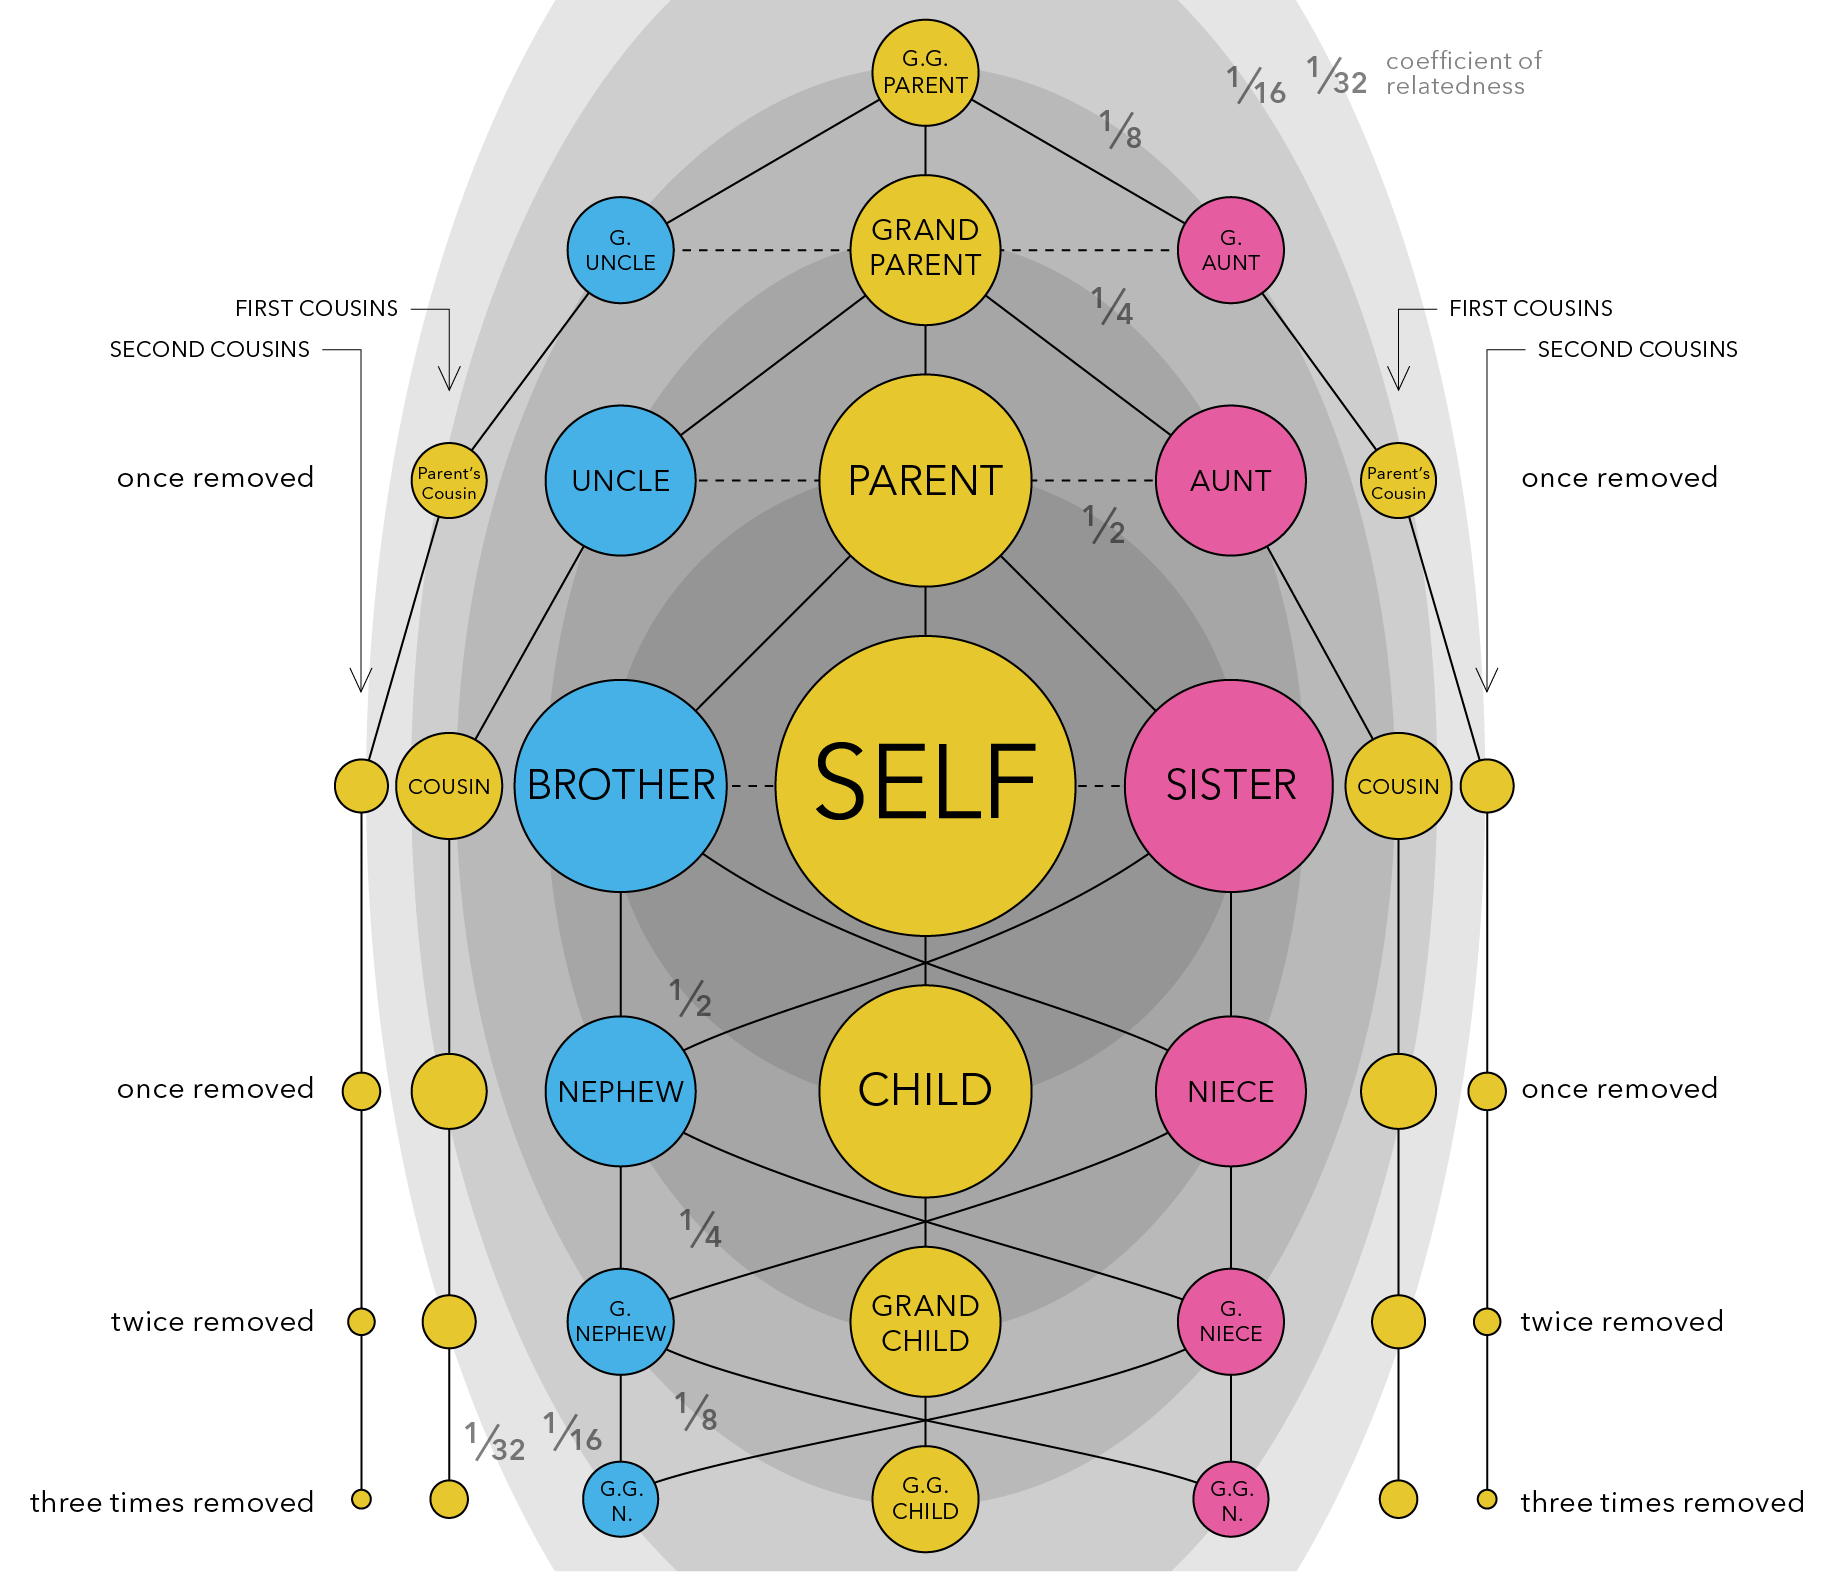
\includegraphics[width=0.5\textwidth]{coefrelate.png}
	\caption{By Citynoise - Own work, CC BY-SA 4.0, \url{https://commons.wikimedia.org/w/index.php?curid=37723128}}
	\label{fig:coefrelate}
\end{figure}
\\ Axelrod and Hamilton~\cite{evolution_of_cooperation} highlight that although the theory works well to explain cooperation between related individual it falls short in explaining the evolution of cooperation between unrelated individuals. This issue also makes it difficult to apply kinship theory as an aid to the evolution of cooperation in multi-agent systems. Kinship theory requires a reproductive drive and metrics for relatedness in order to motivate altruistic acts, both of which would likely be missing in a decentralised multi-agent system.

\subsection{The Iterated Prisoner's Dilemma}
The Iterated Prisoner's Dilemma is one such example of a game-theoretic model that uses direct reciprocity to attempt to solve the problem that the evolution of cooperation puts forward. Direct reciprocity is the idea: ``If I cooperate now, you may cooperate later''~\cite{five_rules_coop}. The Dilemma is, in fact, a game played between two individuals. The game is made up of a number of repeated rounds, in each round the two players can choose between cooperating with or defecting against each other.\\
A payoff matrix is provided such as the one in figure~\ref{fig:payoffmatrix} on page~\pageref{fig:payoffmatrix}. These matrices provide a temptation to defect, but a reward if both players cooperate over multiple rounds. In a single round game it is mathematically best to defect, but in repeated rounds agents are encouraged to cooperate by a mutual gain in score. The mathematics are explained by Martin A. Nowak \textit{et al.} in their paper ``The Arithmetics of Mutual Help''~\cite{arithmetics_of_mutual_help}.\\
The dilemma has been extended into tournaments such as the one in Axelrod and Hamilton~\cite{evolution_of_cooperation}. You can even run tournaments directly in Python using the Axelrod-Python library~\cite{axelrodproject}. Tournaments can come in a variety of styles but the most popular is the round-robin tournament where every player plays a match of the iterated prisoner's dilemma against every other player. Players accumulate points throughout these games, based on the payoff matrix.\\
This has been even further extended to include a genetic algorithm to simulate evolution by reproducing players into the next generation. Multiple different algorithms have been used, one common one is the Moran Process (A stochastic process used to model evolution in a finite, unstructured population) available in the Axelrod-Python library. 
\begin{figure}
	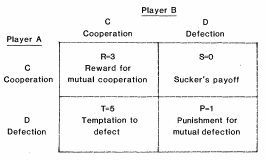
\includegraphics[width=0.5\textwidth]{payoffmatrix.png}
	\caption{The payoff matrix given in Axelrod and Hamilton's paper~\cite{evolution_of_cooperation}}
	\label{fig:payoffmatrix}
\end{figure}

\subsection{Strategies}
Players in the iterated prisoner's dilemma have to be able to decide whether to defect or cooperate in any given round against any given opponent. The player has access to the history of interaction between the two individuals to base their decision on - the simplest of strategies, however, don't use the history, one example being a pure defector.\\
Some more interesting strategies include the world famous tit-for-tat, grudger and Pavlov (win-stay, lose-shift~\cite{nowak-1993a}). The classical form of tit-for-tat begins by cooperating in the first round and then copying the other player's last move, this strategy is so effective because it gives the other player a chance to cooperate (so working well with cooperators) but still punishes a defecting player preventing them from taking advantage. There are many other versions of tit-for-tat, a good example being forgiving tit-for-tat which only defects if the other player defects for two turns in a row.\\
Grudger works by beginning to cooperate but if the other player defects the individual switches and defects for the rest of the time, this is not so effective as tit-for-tat because it never forgives the other player, preventing further cooperation.\\
Pavlov works by continuing to act the way it has in the previous interaction if the action was successful if it is not successful the strategy switches to the other action. Nowak and Sigmund claim that Pavlov outperforms tit-for-tat as tit-for-tat is unsuccessful in non-deterministic environments (such as one that has a random chance that an action will not be what a player chooses). The real world is non-deterministic and so tit-for-tat doesn't generalise into it so well. Pavlov considers a success in a round to be: you both cooperate or you defect and the other player cooperated, and considers a failure to be: you both defect or you cooperate and the other player defects.

\subsection{Other Reciprocation Theories}
Using reciprocity to aid in the evolution of cooperation has not been limited to the iterated prisoner's dilemma. Martin A. Nowak presents 3 other mechanisms that use reciprocation~\cite{five_rules_coop}: indirect reciprocity, network reciprocity (also known as spatial tournaments) and group selection.\\
Indirect Reciprocity is a set of mechanisms that leverage the group mechanic of reputation. Each member of the set of mechanisms uses different metrics for reputation and the spread of information that influences reputation. Nowak and Sigmund's version uses the idea of image scoring~\cite{evol_indirect_image} an image score represents how well an agent is thought of, the higher the better.\\
Which mechanism is more effective is the subject of extensive debate, in two separate papers both Leimar and Hammerstein~\cite{leimarhammer}, and Roberts~\cite{evoldirindir} concluded that the standing strategy is more effective. In the standing strategy agents do not have an image score but have a standing which can be good or bad, everyone starts off with a good standing but if they defect against a player with good standing they are considered to have a bad standing. The spread of information is also key to indirect reciprocity as reputation is directly influenced by the community whereas with direct reciprocity there is no need for this. One mechanism for the spread of information is through gossip~\cite{gossip_alt}.\\
Network reciprocity (also known as spatial tournaments) uses direct reciprocity but not in a round-robin tournament. Spatial tournaments use a graph where nodes are agents and the edges represent channels of connection between agents~\cite{evol_graph}, direct reciprocity games are then played between agents with connections.\\
Nowak and May found that when deployed on a large scale using a reproduction mechanism beautiful spatial patterns can be observed~\cite{spatial}. More importantly, they also found that groups of cooperators can work together to support each other and fend off invasion by defectors - depending on the structure of the graph.\\
Direct Reciprocity is also used in group selection. In this model the population is subdivided into smaller groups, in these smaller groups individuals interact with each other and reproduction occurs from the fitness they gain in these interactions. \\
Though offspring are reproduced into the same group, reproduction occurs on two levels: group sizes fluctuate due to reproduction, if a group gets to a certain size it may split in two and when a group divides another is eliminated to keep the number of groups fixed. Groups with faster reproduction do better than those with slower reproduction. Traulsen and Nowak found this favours the evolution of cooperation under certain conditions~\cite{multilevel_nowak}.

%------------------------------------------------

\section{Discussion and Conclusion}
All these mechanisms to aid in the evolution of cooperation have extremely interesting properties and consequences in both biological and intelligent agents. Network Reciprocity can be used to represent a physical telecommunications network across which agents communicate, group selection is useful to model the spread of successful agent populations displacing others (like the current mass-extinction crisis) and kinship theory is useful to model interactions between different family groups in nature just to name a few applications.\\
With the internet being such a vast medium across which agents may interact it is very likely that agents may not have many repeated meetings, so direct reciprocity is not always applicable. However, agents may often repeat interactions, so indirect reciprocity is not always applicable.\\
Due to the incredible interconnectedness of the internet, the graphs used by network reciprocity would have to be highly connected and this makes it less useful for modelling agent systems using the internet. Due to the lack of reproductive drive and inherent relatedness between agents across the internet Kinship theory is unlikely to apply well.\\
Thus as my project will be aiming to simulate a multi-agent system with agents decentralised across the internet a combination of indirect and direct reciprocity will likely be the most germane aid to the evolution of cooperation for my project.

%----------------------------------------------------------------------------------------
%	REFERENCE LIST
%----------------------------------------------------------------------------------------

\bibliography{../refs.bib}{}
\bibliographystyle{plain}

%----------------------------------------------------------------------------------------

\end{document}
